\documentclass[a4paper,12pt,oneside,openany,table,xcdraw]{article}

\usepackage{setspace}
\usepackage{multirow}
\usepackage{hyperref}
\usepackage{caption}
\usepackage{indentfirst}
\usepackage{tikz} %% fasores
\usetikzlibrary{arrows,arrows.meta,quotes,angles}
\usepackage{siunitx}

\usepackage[brazilian]{babel}
\usepackage[utf8x]{inputenc}
\usepackage{amsmath, graphicx, subfig, enumerate}
\usepackage{float, verbatim}
\usepackage[colorinlistoftodos]{todonotes}
\usepackage{makeidx}
\usepackage{geometry}

\graphicspath{{img/}}
\geometry{a4paper, hmargin={3cm, 3cm}, vmargin={3cm, 2cm} }
\setlength{\parindent}{1.0cm}
\captionsetup{font=small}

\usepackage{mathtools,listings} %%
\usepackage{color} %red, green, blue, yellow, cyan, magenta, black, white
\definecolor{mygreen}{RGB}{28,172,0} % color values Red, Green, Blue
\definecolor{mylilas}{RGB}{170,55,241}
\usepackage{listingsutf8}

\begin{document}
\newcommand{\thedepartment}{Faculdade de Engenharia Elétrica}
\newcommand{\thecourse}{FEELT}
\newcommand{\thetitle}{Resolução da Lista de Exercícios 2}
\newcommand{\thetype}{Trabalho de Princípios de Comunição}
\newcommand{\theproftitle}{Bacharel em Engenharia Elétrica}
\newcommand{\thestudent}{Lesly Viviane Montúfar Berrios\\
\centering11811ETE001}
\newcommand{\theadvisor}{Prof. Lorenço Santos Vasconcelos}
\newcommand{\thecity}{Uberlândia}

\thispagestyle{empty}\newcommand*{\themonth}{\ifthenelse{\the\month < 2}{Janeiro }
                  {\ifthenelse{\the\month < 3}{Fevereiro }
                  {\ifthenelse{\the\month < 4}{Março }
                  {\ifthenelse{\the\month < 5}{Abril }
                  {\ifthenelse{\the\month < 6}{Maio }
                  {\ifthenelse{\the\month < 7}{Junho }
                  {\ifthenelse{\the\month < 8}{Julho }
                  {\ifthenelse{\the\month < 9}{Agosto }
                  {\ifthenelse{\the\month < 10}{Setembro }
                  {\ifthenelse{\the\month < 11}{Outubro }
                  {\ifthenelse{\the\month < 12}{Novembro }{Dezembro }}}}}}}}}}}}
                  
\begin{titlepage}
\begin{center}

	\vspace{-0.5cm}

  \begin{figure}[hbt!]
		\begin{center}
		   
\includegraphics[width=2.8cm]{ufu-logo.png}
		\end{center}
	\end{figure}
 	%\vspace{-4cm}

%\begin{doublespacing}

  \Large{\textbf{Universidade Federal de Uberlândia}}\\
  \large{\thedepartment}\\
  \large{\thecourse}\\


\vspace{5.8cm}
  \par
  \large\textbf{\thetitle}
\vspace{5.8cm} 

%\end{doublespacing}
  \par
  \thetype\\
  por\\
  %\hspace{2cm}\large{}\\

\vspace{0.8cm}
\par
  \normalsize{\thestudent}\\ [2cm]
  \theadvisor

\par\vfill
  \thecity, \themonth / \the\year

\end{center}

\end{titlepage}

\lstset{language=Matlab,%
	inputencoding=utf8/latin1,
    %basicstyle=\color{red},
    breaklines=true,%
    morekeywords={matlab2tikz},
    keywordstyle=\color{blue},%
    morekeywords=[2]{1}, keywordstyle=[2]{\color{black}},
    identifierstyle=\color{black},%
    stringstyle=\color{mylilas},
    commentstyle=\color{mygreen},%
    showstringspaces=false,%without this there will be a symbol in the places where there is a space
    numbers=left,%
    numberstyle={\tiny \color{black}},% size of the numbers
    numbersep=9pt, % this defines how far the numbers are from the text
    emph=[1]{for,end,break},emphstyle=[1]\color{red}, %some words to emphasise
    %emph=[2]{word1,word2}, emphstyle=[2]{style},    
}

%% Comeca o documento !

\onehalfspacing
\tableofcontents % sumário
\newpage

\section{Exercício 1}
É apresentado um circuito modulador e a análise é feita pelo código do anexo Anexo \ref{anexo:ex1}. O gráfico o sinal modeulante $m(t)$ e da portadora $c(t)$ é apresentado na Figura \ref{1:sinais}. As tensões $v_1(t)$ e $v_2(t)$, na saída do somador e do diodo respectivamente, possuem comportamento descrito na Figura \ref{1:v1_v2}. O espectro do sinal $v_1(t)$, $v_2(t)$ e $y(t)$ (sinal modulado) estão ilustrados nas Figuras \ref{1:fft:v1}, \ref{1:fft:v2} e \ref{1:fft:saida}.

\vspace{0.5cm}
\begin{figure}[H]
\centering
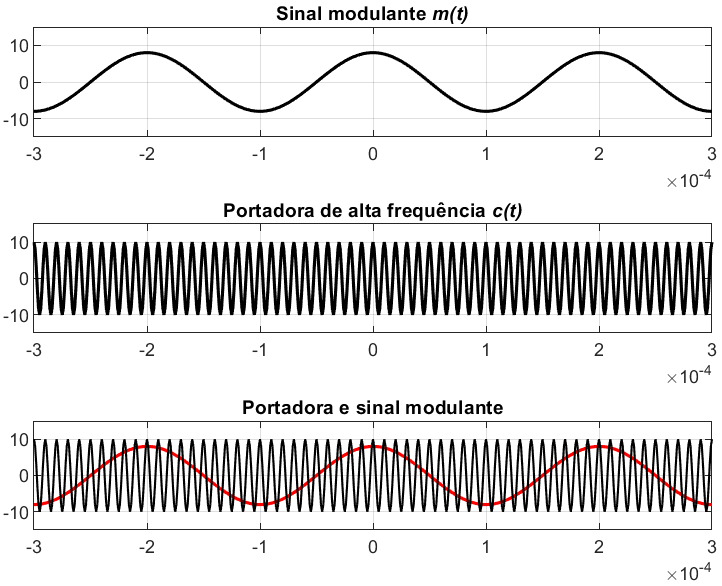
\includegraphics[width=\textwidth]{ex1}
\caption{Sinal modulante $m(t)$ e da portadora $c(t)$.}
\label{1:sinais}
\end{figure}

\vspace{0.3cm}
\begin{figure}[H]
\centering
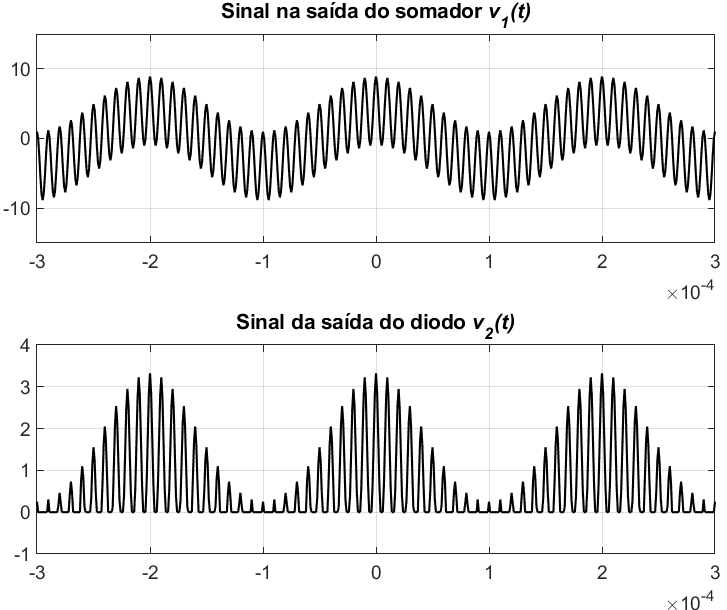
\includegraphics[width=\textwidth]{ex1_v1_v2}
\caption{Sinal de tensão no ponto 1, $v_1(t)$, e no ponto 2, $v_2(t)$.}
\label{1:v1_v2}
\end{figure}

\vspace{0.3cm}
\begin{figure}[H]
\centering
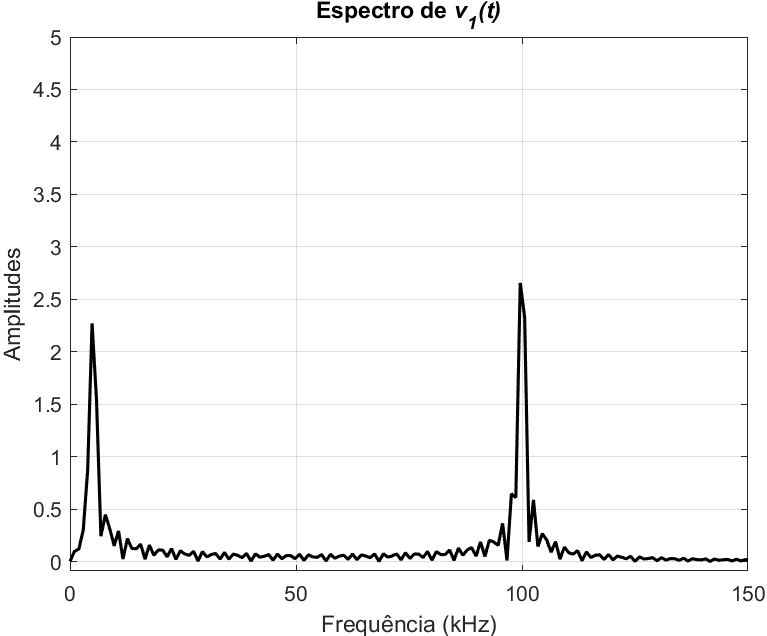
\includegraphics[width=\textwidth]{ex1_espectro_v1}
\caption{Espectro de frequência na saída do somador.}
\label{1:fft:v1}
\end{figure}

\vspace{0.3cm}
\begin{figure}[H]
\centering
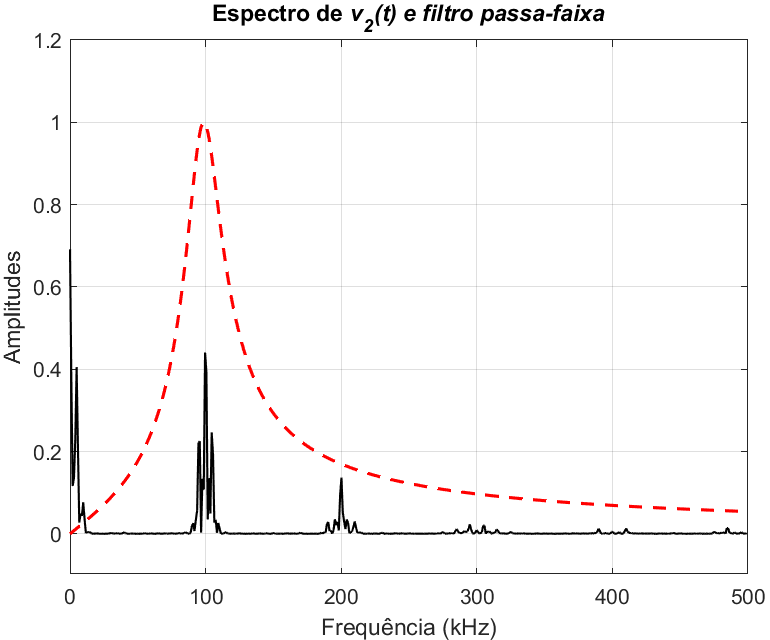
\includegraphics[width=\textwidth]{ex1_espectro_v2}
\caption{Espectro de frequência na saída do diodo.}
\label{1:fft:v2}
\end{figure}

\vspace{0.3cm}
\begin{figure}[H]
\centering
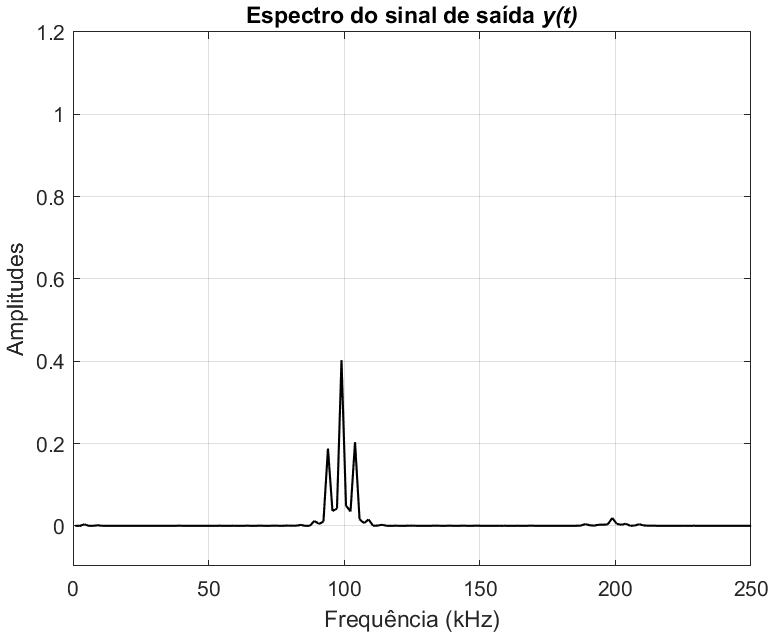
\includegraphics[width=\textwidth]{ex1_espectro_saida}
\caption{Espectro de frequência na saída do diodo.}
\label{1:fft:saida}
\end{figure}

\vspace{0.3cm}
\begin{figure}[H]
\centering
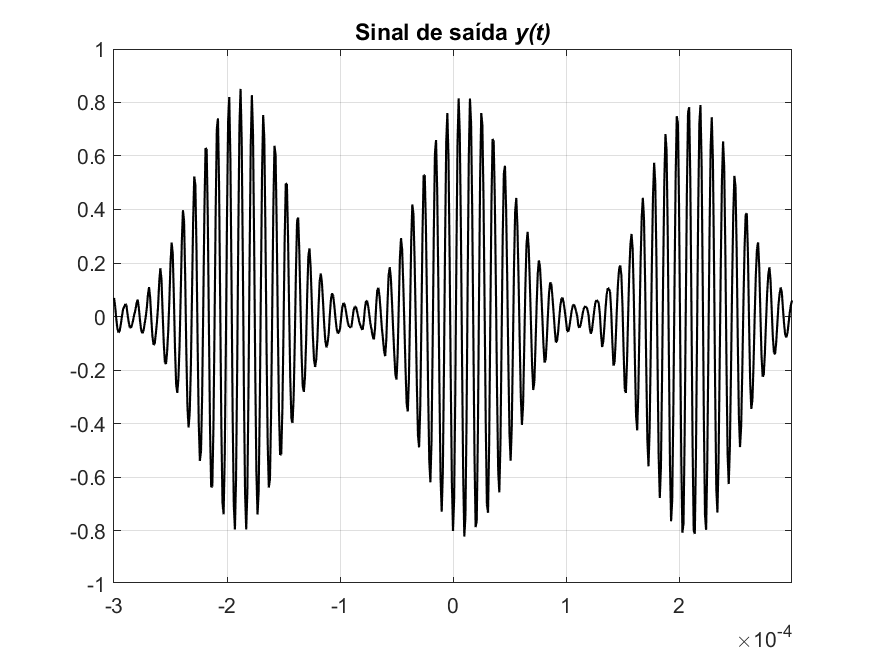
\includegraphics[width=\textwidth]{ex1_yt}
\caption{Sinal modulado.}
\label{1:fft:saida}
\end{figure}


\newpage
\section{Exercício 2}
Usando o demodulador apresentado com $C=10nF$ obtém-se os gráficos das Figuras \ref{2:1}, \ref{2:2}, \ref{2:3} e  \ref{2:4}.

\vspace{0.3cm}
\begin{figure}[H]
\centering
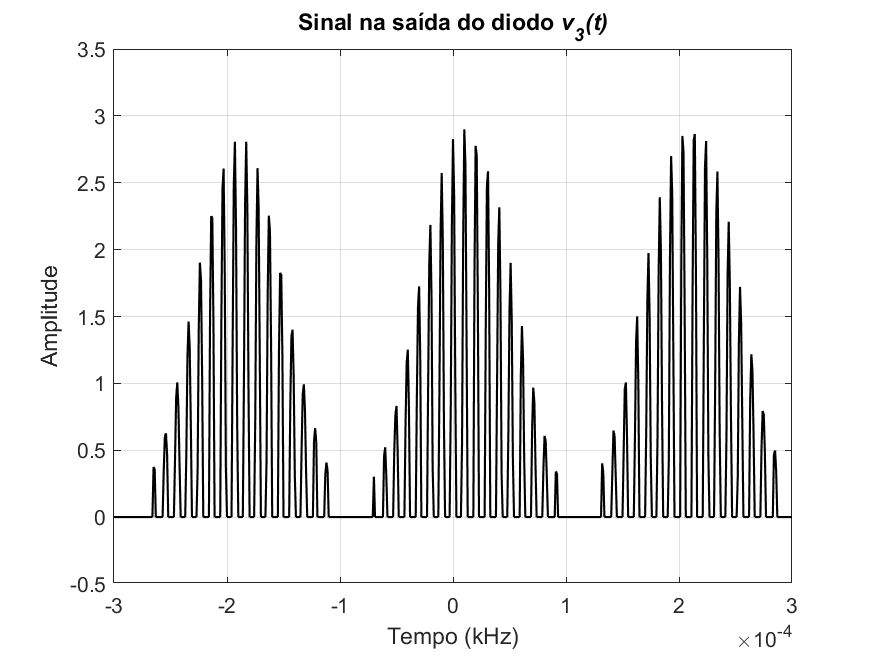
\includegraphics[width=\textwidth]{ex2_diodo}
\caption{Sinal de saída do diodo.}
\label{2:1}
\end{figure}

\vspace{0.3cm}
\begin{figure}[H]
\centering
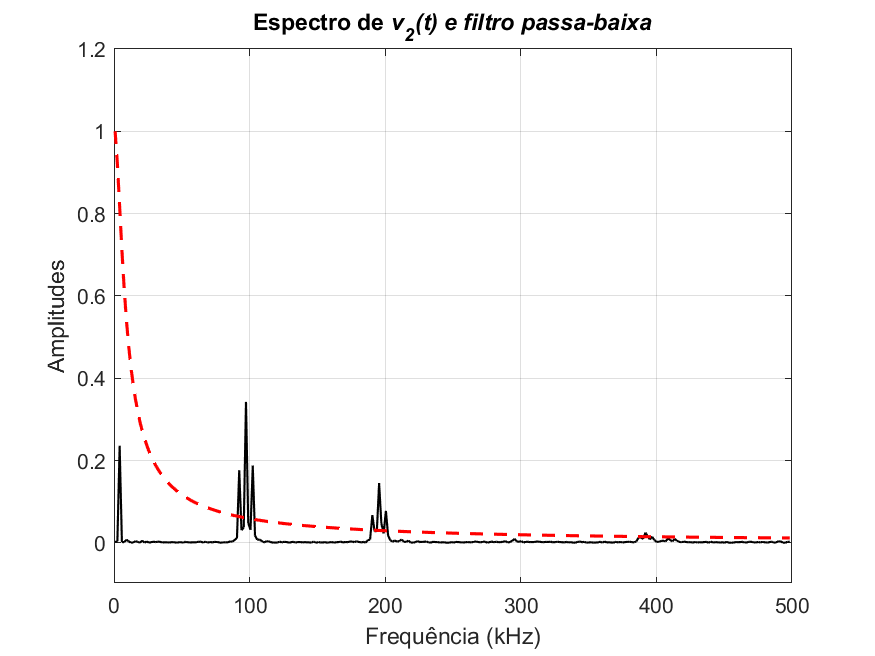
\includegraphics[width=\textwidth]{ex2_espectro_diodo}
\caption{Espectro do sinal de saída do diodo.}
\label{2:2}
\end{figure}

\vspace{0.3cm}
\begin{figure}[H]
\centering
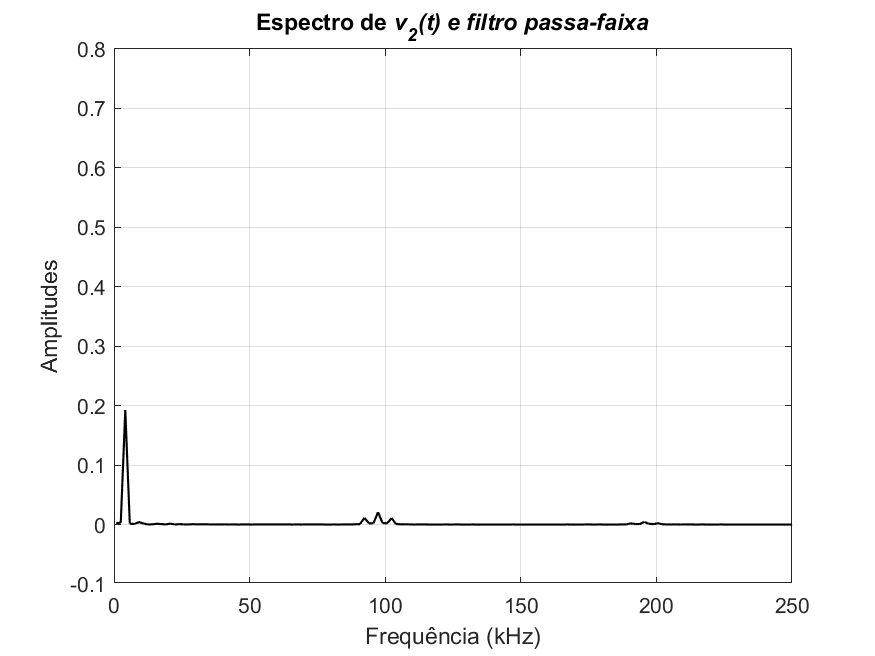
\includegraphics[width=\textwidth]{ex2_espectro_saida}
\caption{Espectro do sinal de saída.}
\label{2:3}
\end{figure}

\vspace{0.3cm}
\begin{figure}[H]
\centering
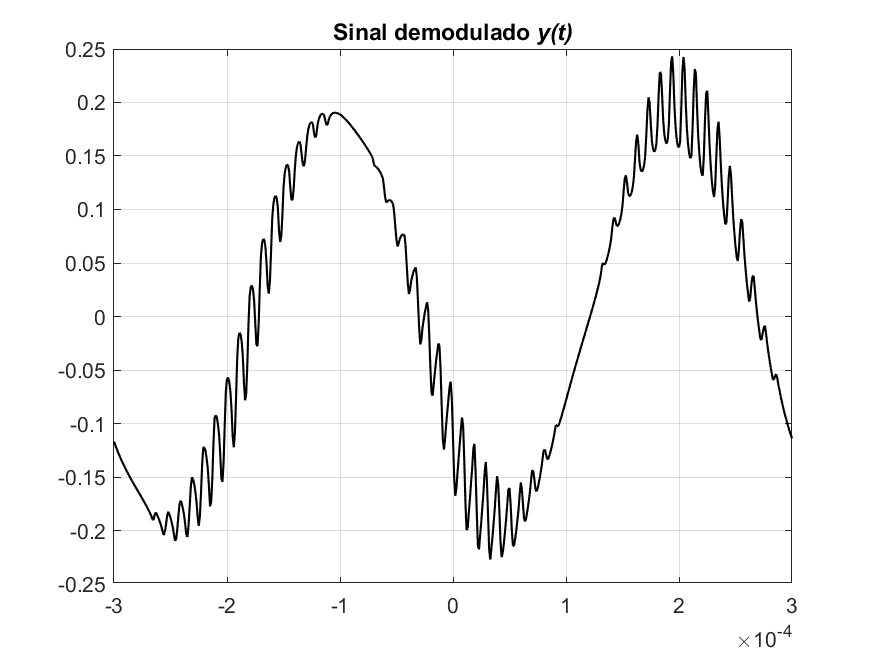
\includegraphics[width=\textwidth]{ex2_saida}
\caption{Sinal de saída no tempo.}
\label{2:4}
\end{figure}

\newpage
Usando o demodulador apresentado com $C=1nF$ obtém-se os gráficos das Figuras \ref{22:1}, \ref{22:2}, \ref{22:3} e  \ref{22:4}.

\vspace{0.3cm}
\begin{figure}[H]
\centering
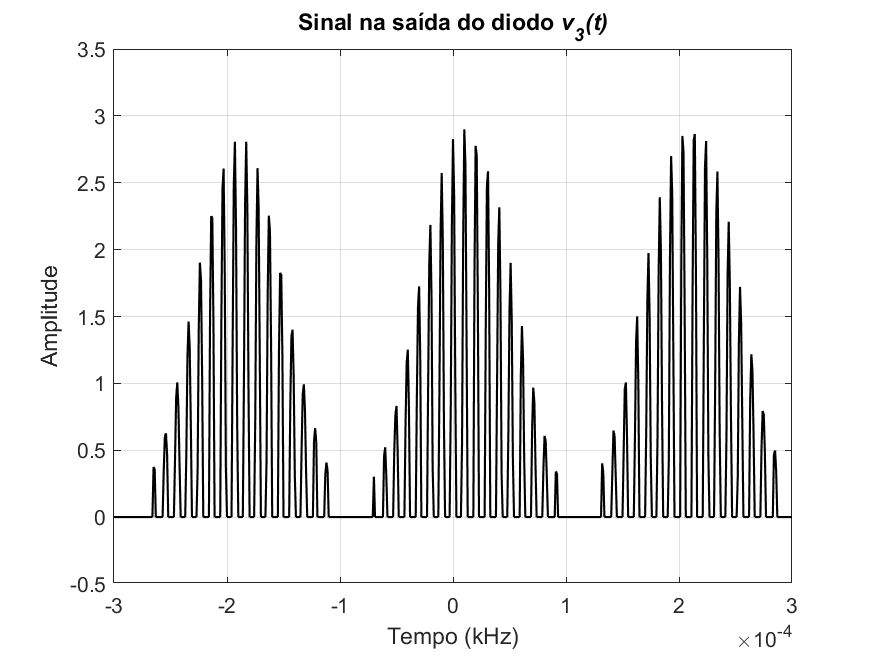
\includegraphics[width=\textwidth]{ex2_diodo_2}
\caption{Sinal de saída do diodo.}
\label{22:1}
\end{figure}

\vspace{0.3cm}
\begin{figure}[H]
\centering
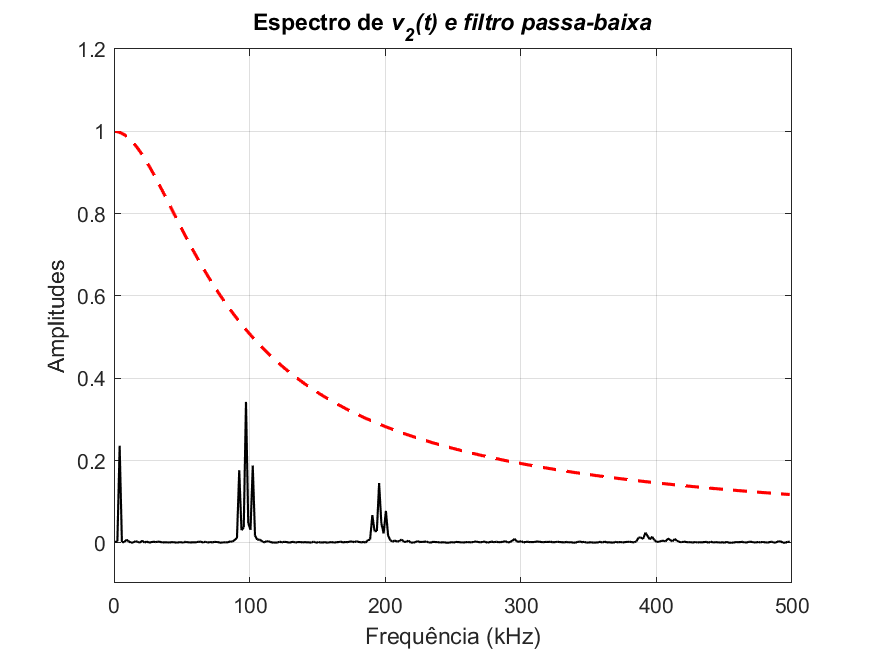
\includegraphics[width=\textwidth]{ex2_espectro_diodo_2}
\caption{Espectro do sinal de saída do diodo.}
\label{22:2}
\end{figure}

\vspace{0.3cm}
\begin{figure}[H]
\centering
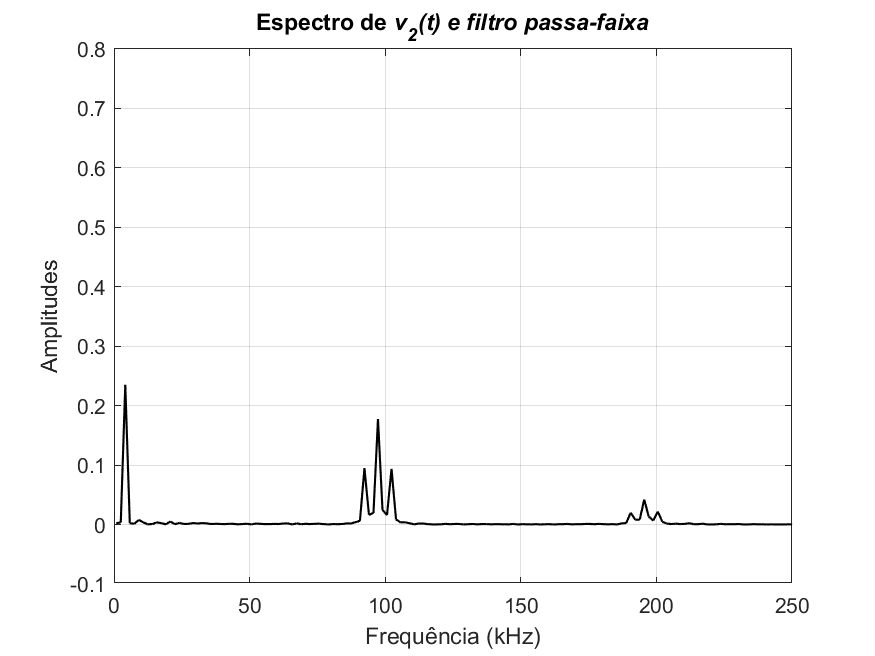
\includegraphics[width=\textwidth]{ex2_espectro_saida_2}
\caption{Espectro do sinal de saída.}
\label{22:3}
\end{figure}

\vspace{0.3cm}
\begin{figure}[H]
\centering
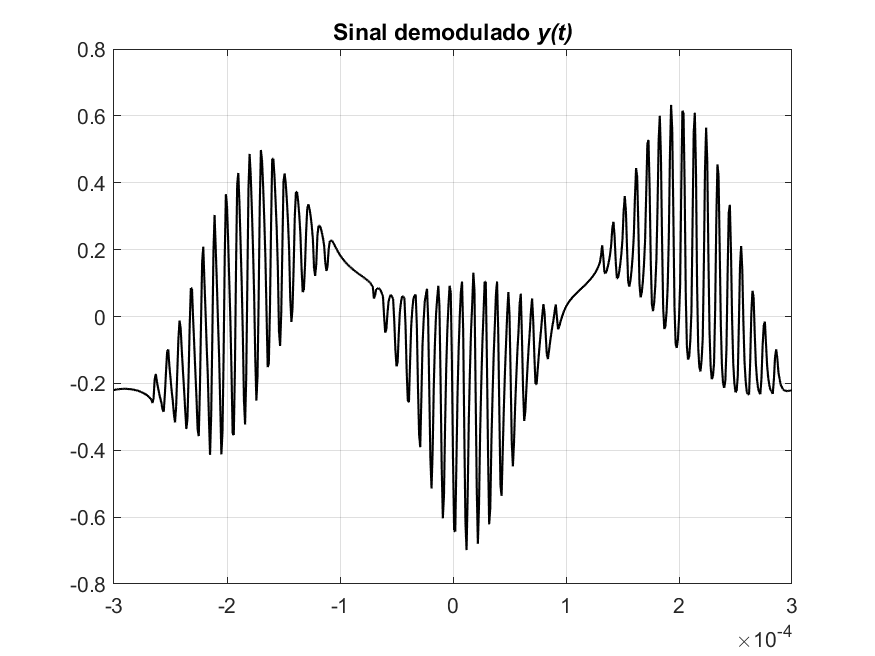
\includegraphics[width=\textwidth]{ex2_saida_2}
\caption{Sinal de saída no tempo.}
\label{22:4}
\end{figure}

\newpage
Usando o demodulador apresentado com $C=120nF$ obtém-se os gráficos das Figuras \ref{23:1}, \ref{23:2}, \ref{23:3} e  \ref{23:4}.

\vspace{0.3cm}
\begin{figure}[H]
\centering
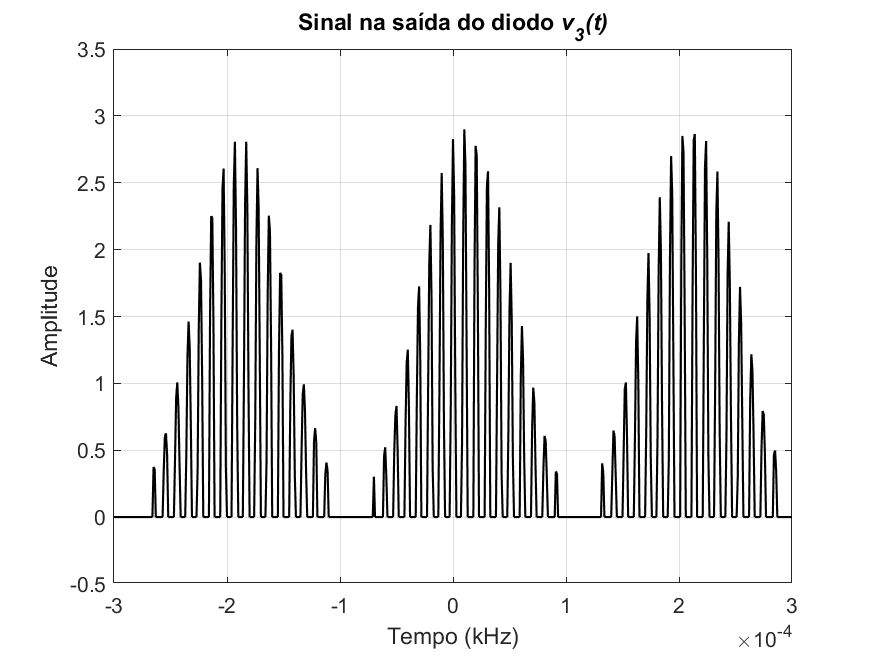
\includegraphics[width=\textwidth]{ex2_diodo_3}
\caption{Sinal de saída do diodo.}
\label{23:1}
\end{figure}

\vspace{0.3cm}
\begin{figure}[H]
\centering
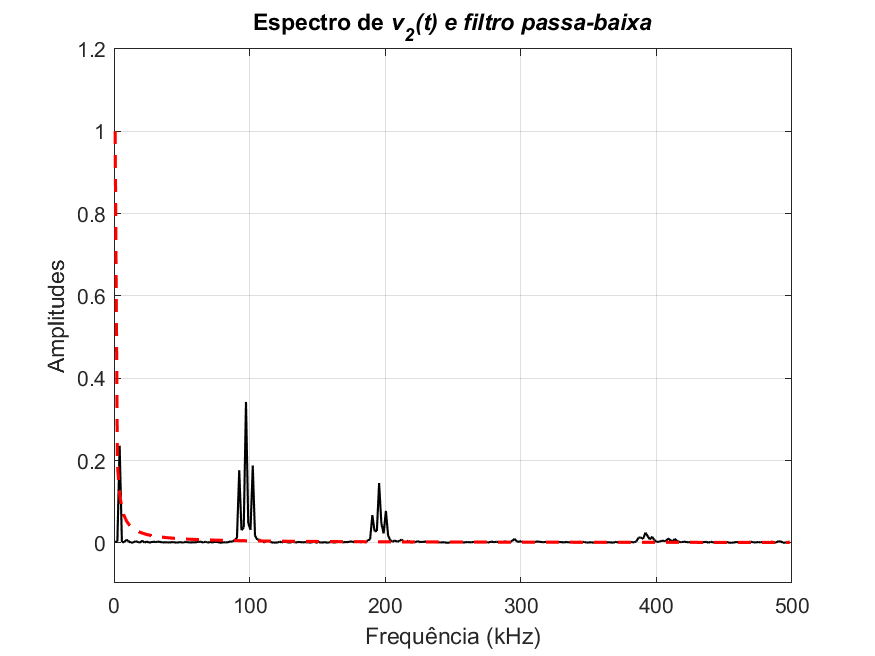
\includegraphics[width=\textwidth]{ex2_espectro_diodo_3}
\caption{Espectro do sinal de saída do diodo.}
\label{23:2}
\end{figure}

\vspace{0.3cm}
\begin{figure}[H]
\centering
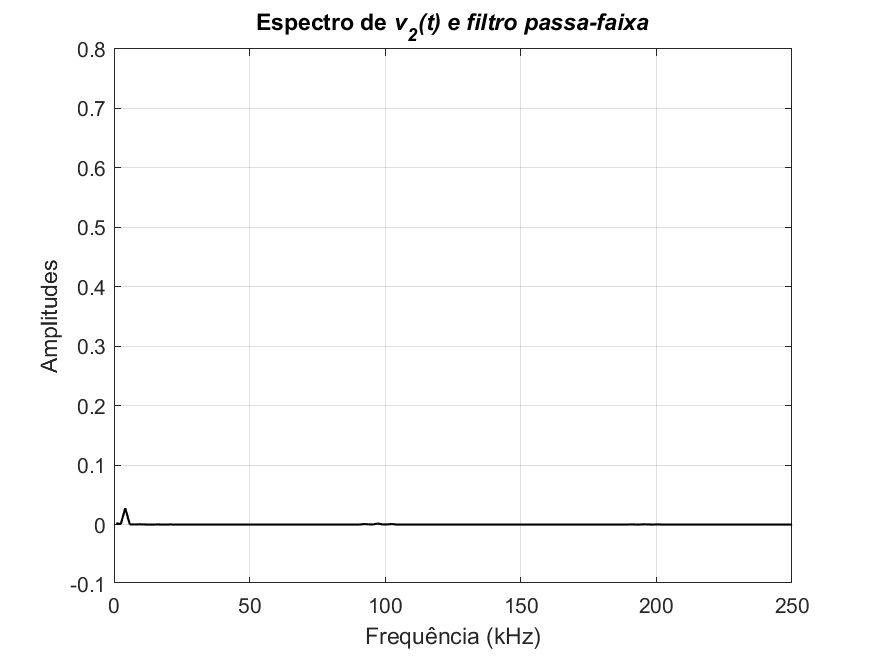
\includegraphics[width=\textwidth]{ex2_espectro_saida_3}
\caption{Espectro do sinal de saída.}
\label{23:3}
\end{figure}

\vspace{0.3cm}
\begin{figure}[H]
\centering
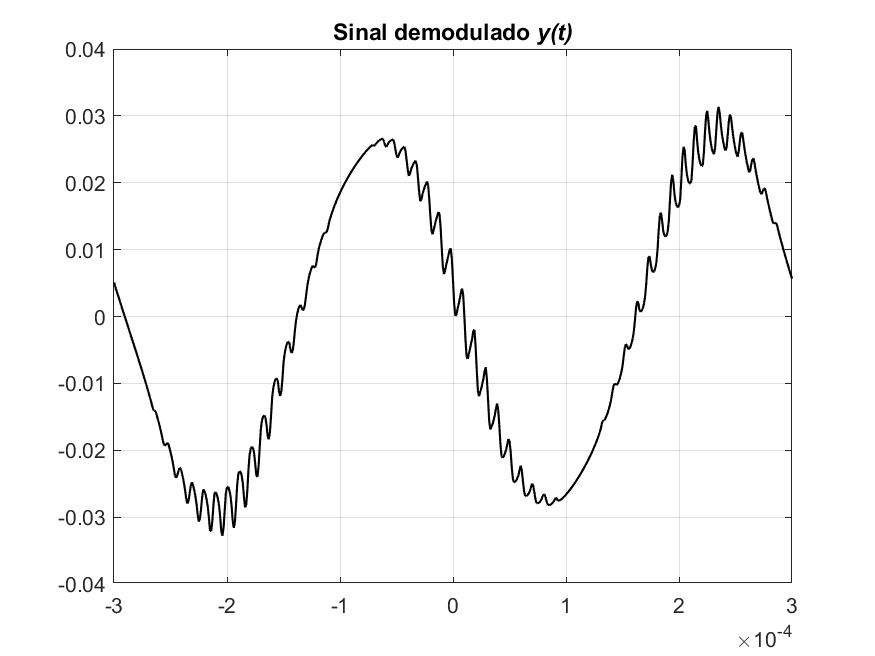
\includegraphics[width=\textwidth]{ex2_saida_3}
\caption{Sinal de saída no tempo.}
\label{23:4}
\end{figure}
 
\newpage
\section{Anexos}
\subsection{Código correspondente ao exercício 1 e 2} \label{anexo:ex1}
\lstinputlisting{codes/EX1.m}

%\vspace{0.3cm}
%\subsection{Código correspondente ao exercício 2} \label{anexo:ex2}
%\lstinputlisting{codes/EX2.m}

\newpage
\begin{thebibliography}{9} 
% Introdução
%\bibitem{S1}
%    Gene F. Franklin, J. David Powell, Abbas Emami-Naieni.,
%    “Sistemas de Controle para a Engenharia”, Porto Alegre: Bookman, 2013.

%\bibitem{S2}
%    Oppeinheim, Alan V.; Willsky, Allan S.,
%    “Sinais e Sistemas”, São Paulo: Pearson
%Prentice Hall, 2010. 2ª Edição.

\bibitem{S2}
    Lathi, B. P.; Ding, Zhi,
    “Modern Digital and Analog Communication Systems”, New York: 
    Oxford University Press, 2019. 5ª Edição.

\end{thebibliography}
\end{document}
